\documentclass[journal]{IEEEtran}

\usepackage{tabularx}
\usepackage{graphicx} % Required for inserting images
\usepackage{cite}
\usepackage{amsmath,amssymb,amsfonts}
\usepackage{algorithmic}
\usepackage{graphicx}
\usepackage{textcomp}
\usepackage{xcolor}
\usepackage{hyperref}
\usepackage{subfig}
\usepackage{wrapfig}

\title{ML Challenge Report}
\author{
  Siqi Liu
  \and
  Rafay Usman
  \and
  Ryan Shiels
  \and
  Albert Li
}
\date{April 2025}

\begin{document}

\maketitle

\section{Models}
% A description of the model(s) that you are evaluating/exploring. We are expecting a thorough
% exploration of at least 3+ family of models1, even if you don’t ultimately use those models. We are looking for:
% – How you are applying these models. You don’t need to reiterate what the models are and how they work. Instead, we’re looking for a description of the choices you are making to apply the model to this task: e.g., what features from the “Data” section are you using for each model? What adjustments (if any) did you need to make?

The setup of our training is similar for all models:
% Make a bullet point list
\begin{itemize}
\item We used the cleaned and encoded data as described in \ref{sec:exploration}.
\item We split the data into training, validation and test sets using a 60/20/20 split using \href{https://scikit-learn.org/stable/modules/generated/sklearn.model_selection.train_test_split.html}{train\_test\_split} from sklearn. We used a consistent random seed of 42 to ensure reproducibility.
\item We used stratified sampling to ensure that the distribution of classes is similar in both sets.
\item We used the same evaluation metrics for all models: accuracy, precision, recall, and F1-score.
\item We used \href{https://rasbt.github.io/mlxtend/user_guide/evaluate/bias_variance_decomp/}{bias\_variance\_decomp} from mlxtend to calculate the bias and variance of our models.
\item We used \href{https://scikit-learn.org/stable/modules/generated/sklearn.metrics.classification_report.html}{classification\_report} from sklearn to generate the classification report for our models.

\subsection{Neural Network}

We started with training a MLPClassifier on the cleaned and encoded data as described in \ref{sec:exploration} using the default parameters by
\href{https://scikit-learn.org/stable/modules/generated/sklearn.neural_network.MLPClassifier.html}{sklearn}.
The default configuration is as follows:
Hidden layer: 1 layer, 100 hidden units
Activation: ReLu
We achieved an 90\% validation accuracy with this base configuration without any tuning, and 87\% on the test set.
We have also tested bagged models and normalization. Specifically, we used the sklearn \href{https://scikit-learn.org/stable/modules/generated/sklearn.ensemble.BaggingClassifier.html}{BaggingClassifier}
with MLPClassifier as the estimator with 10 estimators. As we learned in class, we expected the bagged model to have lower variance because the prediction is the average of many MLPClassifiers.
This is confirmed when we performed variance bias decomposition as seen in \ref{tab:nn_bias_var}, where the bagged model has a lower variance than the non-bagged model.
We also tried normalizing the data using the \href{https://scikit-learn.org/stable/modules/generated/sklearn.preprocessing.StandardScaler.html}{StandardScaler} from sklearn.
We expected normalization to help the model converge faster and prevent overfitting, but it did not have a significant impact on the model accuracy.
We think this is because the data was already cleaned and encoded, and the features were already in a similar range.
For example, the numerical features like "How much would you expect to pay" already have similar ranges (5-20) as the categorical features like "How many ingredients would you expect to be in the food".

\begin{table}[ht]
    \centering
    \begin{tabular}{lccc}
        \hline
        Model                  & Expected Loss & Bias   & Variance \\
        \hline
        MLP                    & 0.1356        & 0.1155 & 0.0638   \\
        Bagging MLP            & 0.1362        & 0.1277 & 0.0543   \\
        Normalized MLP         & 0.1368        & 0.1185 & 0.0628   \\
        Normalized Bagging MLP & 0.1384        & 0.1337 & 0.0530   \\
        \hline
    \end{tabular}
    \caption{Loss, Bias, and Variance for Different Models}
    \label{tab:nn_bias_var}
\end{table}

\ref{tab:nn_classification_report} shows the classification report for the MLPClassifier.
The model performed well on the validation set, with an accuracy of 90\% and a balanced precision and recall across all classes.
The F1-score for all classes was around 0.90, indicating a good balance between precision and recall.

\begin{table}[ht]
    \centering
    \begin{tabular}{lcccc}
        \hline
        Category     & Precision & Recall & F1-score & Support \\
        \hline
        Pizza        & 0.92      & 0.90   & 0.91     & 88      \\
        Shawarma     & 0.87      & 0.91   & 0.89     & 88      \\
        Sushi        & 0.91      & 0.89   & 0.90     & 87      \\
        \hline
        Accuracy     &           &        & 0.90     & 263     \\
        Macro avg    & 0.90      & 0.90   & 0.90     & 263     \\
        Weighted avg & 0.90      & 0.90   & 0.90     & 263     \\
        \hline
    \end{tabular}
    \caption{Classification Report for Pizza, Shawarma, and Sushi}
    \label{tab:nn_classification_report}
\end{table}


\subsection{Decision Trees}
I tested a regular decision tree, an ensemble of decision trees, and a Random Forest model, using the built-in RandomForestClassifier from sklearn. I found the decision tree to perform the worst, and it was easier to manipulate the RandomForestClassifier’s parameters, so I decided to explore that further.

I decided to include all of the possible features (even initially 'id' accidentally), as the Random Forest was very robust regardless of the feature choice or hyperparameters. To allow the text-based features to generalize as well as possible, I used a library to cluster text by Levenshtein distance, and to limit overfitting, I only included the categories with enough representatives. This did not seem to have too large an impact on validation accuracy, but would allow it to correctly categorize otherwise unseen data with unique typos or spelling choices.
I tested many of the hyperparameter options, but found little change in accuracy aside from increasing the number of estimators to around 250, and limiting the minimum samples split to 10. Some randomness was introduced when generating text clusters, but I found it to still be very consistently accurate regardless of what data it trained on.

It consistently achieved an 87\% validation accuracy. The classification report initially showed it was particularly effective at identifying Pizza and Shawarma, but had some difficulty with Sushi, which I would expect if respondents have less familiarity with Sushi. However, after splitting the training data such that there is the same amount of each in the training and validation portions, this was no longer the case.
\begin{table}[ht]
    \centering
    \begin{tabular}{lccc}
        \hline
        Category     & Precision                              & Recall & F1-score \\
        \hline
        Pizza        & 0.85                                   & 0.93   & 0.89     \\
        Shawarma     & 0.88                                   & 0.84   & 0.86     \\
        Sushi        & 0.90                                   & 0.86   & 0.88     \\
        \hline
        Accuracy     & \multicolumn{3}{c}{0.88 (263 samples)}                     \\
        Macro avg    & 0.88                                   & 0.88   & 0.88     \\
        Weighted avg & 0.88                                   & 0.88   & 0.88     \\
        \hline
    \end{tabular}
    \caption{Classification Report}
    \label{tab:classification_report}
\end{table}

After comparing the loss, bias, variance decomposition to our other models, I found the expected higher bias, but lower variance that Random Forests are known to have:
\begin{table}[ht]
    \centering
    \begin{tabular}{ccc}
        \hline
        Loss   & Bias   & Variance \\
        \hline
        0.1380 & 0.1255 & 0.0410   \\
        \hline
    \end{tabular}
    \label{tab:loss_report}
\end{table}

\subsection{Word Embedding - Neural Network}
We implemented a feedforward neural network with three hidden layers consisting of 64, 64, and 64 neurons, respectively. The hidden layers utilized ReLU activation functions, while the output layer employed a softmax activation function. The model was trained using a learning rate of 0.001 and a batch size of 32, with categorical cross-entropy as the loss function. Training was conducted over 300 epochs, achieving a validation accuracy of approximately 84\%. For feature selection, we used word similarity embeddings for questions Q5, Q6, and Q7. For Q1, Q2, and Q4, we computed the average of all numerical values in the text, and for Q3 and Q8, we employed one-hot encoded categorical vectors.

We experimented with various configurations of the model, including adjustments to the number of hidden layers, neurons per layer, and activation functions. For activation functions, we tested leaky ReLU, sigmoid, and tanh. While leaky ReLU and tanh achieved validation accuracies of 82\% and 84\% respectively, the sigmoid function performed significantly worse, achieving only 65\%.

We also explored different hidden layer configurations. Increasing the number of neurons to 128, 64, and 64 per layer slightly reduced the accuracy to 82\% and increased training time. Reducing the neurons to 32, 16, and 16 per layer also resulted in a lower accuracy of 82\%. A configuration of 32 neurons in each of the three layers yielded a similar accuracy of 82\%.

Additionally, we tested varying the number of hidden layers while keeping each layer at 64 neurons. Reducing the number of layers to 1 or 2 led to validation accuracies of 82\% and 83\%, respectively. Increasing the number of layers to 4 or 5 did not improve performance, maintaining an accuracy of 84\%.

\begin{table}[h]
    \centering
    \begin{tabular}{lccc}
        \hline
        Category     & Precision                              & Recall & F1-score \\
        \hline
        Pizza        & 0.86                                   & 0.83   & 0.85     \\
        Shawarma     & 0.85                                   & 0.85   & 0.85     \\
        Sushi        & 0.82                                   & 0.85   & 0.83     \\
        \hline
        Accuracy     & \multicolumn{3}{c}{0.84 (329 samples)}                     \\
        Macro avg    & 0.84                                   & 0.84   & 0.84     \\
        Weighted avg & 0.84                                   & 0.84   & 0.84     \\
        \hline                                                                    \\
    \end{tabular}
    \begin{tabular}{ccc}
        \hline
        Loss   & Bias   & Variance \\
        \hline
        0.2269 & 0.2269 & 0.0731   \\
        \hline                     \\
    \end{tabular}
    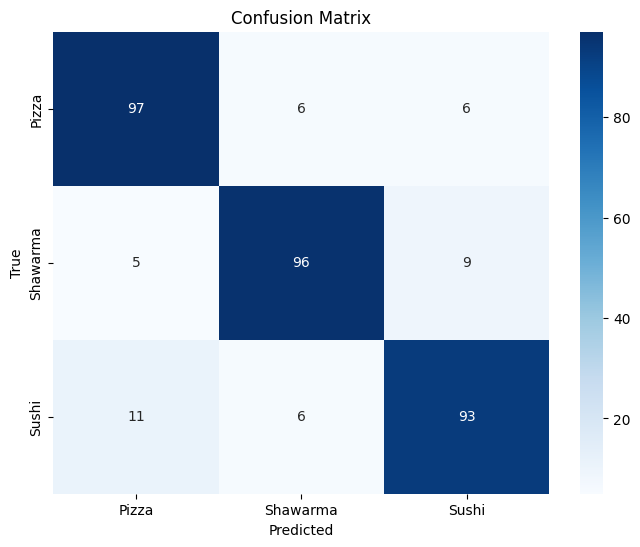
\includegraphics[width=0.45\textwidth]{model/neuralnetwork_confusion.png}
    \caption{Word Embedding Neural Network}
\end{table}

\subsection{Word Embedding - Linear Regression}
We also evaluated a linear regression model. The implementation leveraged sklearn's Linear Regression module, utilizing the same feature set as the neural network. The model achieved a validation accuracy of approximately 86\%, demonstrating competitive performance. This comparison with the neural network revealed that the simpler linear regression model performed slightly better, suggesting that the features representing the dataset may not exhibit significant complexity.

We tested multiple hyperparameter including setting `fit\_intercept' to False and `positive' to False. Setting `fit\_intercept' to False resulted in a lower accuracy of 0.85\%, while setting `positive' to False yielded the same accuracy as the default setting.

\begin{table}[h]
    \centering
    \begin{tabular}{lccc}
        \hline
        Category     & Precision                              & Recall & F1-score \\
        \hline
        Pizza        & 0.86                                   & 0.89   & 0.87     \\
        Shawarma     & 0.89                                   & 0.87   & 0.88     \\
        Sushi        & 0.86                                   & 0.85   & 0.85     \\
        \hline
        Accuracy     & \multicolumn{3}{c}{0.87 (329 samples)}                     \\
        Macro avg    & 0.87                                   & 0.87   & 0.87     \\
        Weighted avg & 0.87                                   & 0.87   & 0.87     \\
        \hline                                                                    \\
    \end{tabular}
    \begin{tabular}{ccc}
        \hline
        Loss   & Bias   & Variance \\
        \hline
        0.2515 & 0.2515 & 0.0088   \\
        \hline                     \\
    \end{tabular}
    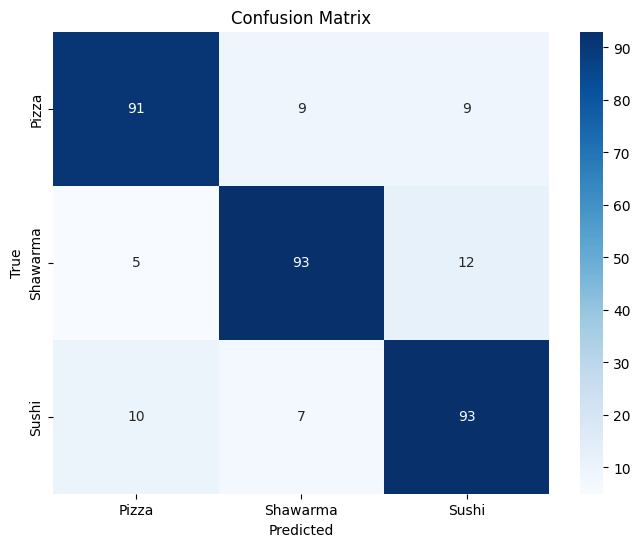
\includegraphics[width=0.45\textwidth]{model/linearregression_confusion.png}
    \caption{Word Embedding Linear Regression}
\end{table}

\subsection{Comparison of Word Embedding Models with Other Approaches}
The Word Embedding Neural Network yielded an accuracy of about 84\%, with a loss of 0.2269, a bias equal to its loss (0.2269), and a variance of 0.0731. The high bias suggests that it does not capture all complexity, while the variance stays relatively moderate. The Word Embedding Linear Regression achieved a slightly higher accuracy at 86\%, accompanied by a loss of 0.2515, bias of 0.2515, and a notably lower variance of 0.0088. Though its loss was higher, the overall bias-variance profile indicates more stable predictions compared to the neural network variant.

Compared to other models such as the MLPClassifier (90\% accuracy) and RandomForestClassifier (87\% accuracy), these word embedding approaches showed somewhat lower accuracies. The neural network had a higher variance component, while the regression model leaned toward higher bias. They both demonstrate that the selected text-based features might not require very deep representations, and simpler linear methods can yield competitive results. The neural network's complexity may not be justified given the representation of the dataset, as indicated by the performance of the linear regression model.

\section{Models}
% A description of the model(s) that you are evaluating/exploring. We are expecting a thorough
% exploration of at least 3+ family of models1, even if you don’t ultimately use those models. We are looking for:
% – How you are applying these models. You don’t need to reiterate what the models are and how they work. Instead, we’re looking for a description of the choices you are making to apply the model to this task: e.g., what features from the “Data” section are you using for each model? What adjustments (if any) did you need to make?

The setup of our training is similar for all models:
% Make a bullet point list
\begin{itemize}
\item We used the cleaned and encoded data as described in \ref{sec:exploration}.
\item We split the data into training, validation and test sets using a 60/20/20 split using \href{https://scikit-learn.org/stable/modules/generated/sklearn.model_selection.train_test_split.html}{train\_test\_split} from sklearn. We used a consistent random seed of 42 to ensure reproducibility.
\item We used stratified sampling to ensure that the distribution of classes is similar in both sets.
\item We used the same evaluation metrics for all models: accuracy, precision, recall, and F1-score.
\item We used \href{https://rasbt.github.io/mlxtend/user_guide/evaluate/bias_variance_decomp/}{bias\_variance\_decomp} from mlxtend to calculate the bias and variance of our models.
\item We used \href{https://scikit-learn.org/stable/modules/generated/sklearn.metrics.classification_report.html}{classification\_report} from sklearn to generate the classification report for our models.

\subsection{Neural Network}

We started with training a MLPClassifier on the cleaned and encoded data as described in \ref{sec:exploration} using the default parameters by
\href{https://scikit-learn.org/stable/modules/generated/sklearn.neural_network.MLPClassifier.html}{sklearn}.
The default configuration is as follows:
Hidden layer: 1 layer, 100 hidden units
Activation: ReLu
We achieved an 90\% validation accuracy with this base configuration without any tuning, and 87\% on the test set.
We have also tested bagged models and normalization. Specifically, we used the sklearn \href{https://scikit-learn.org/stable/modules/generated/sklearn.ensemble.BaggingClassifier.html}{BaggingClassifier}
with MLPClassifier as the estimator with 10 estimators. As we learned in class, we expected the bagged model to have lower variance because the prediction is the average of many MLPClassifiers.
This is confirmed when we performed variance bias decomposition as seen in \ref{tab:nn_bias_var}, where the bagged model has a lower variance than the non-bagged model.
We also tried normalizing the data using the \href{https://scikit-learn.org/stable/modules/generated/sklearn.preprocessing.StandardScaler.html}{StandardScaler} from sklearn.
We expected normalization to help the model converge faster and prevent overfitting, but it did not have a significant impact on the model accuracy.
We think this is because the data was already cleaned and encoded, and the features were already in a similar range.
For example, the numerical features like "How much would you expect to pay" already have similar ranges (5-20) as the categorical features like "How many ingredients would you expect to be in the food".

\begin{table}[ht]
    \centering
    \begin{tabular}{lccc}
        \hline
        Model                  & Expected Loss & Bias   & Variance \\
        \hline
        MLP                    & 0.1356        & 0.1155 & 0.0638   \\
        Bagging MLP            & 0.1362        & 0.1277 & 0.0543   \\
        Normalized MLP         & 0.1368        & 0.1185 & 0.0628   \\
        Normalized Bagging MLP & 0.1384        & 0.1337 & 0.0530   \\
        \hline
    \end{tabular}
    \caption{Loss, Bias, and Variance for Different Models}
    \label{tab:nn_bias_var}
\end{table}

\ref{tab:nn_classification_report} shows the classification report for the MLPClassifier.
The model performed well on the validation set, with an accuracy of 90\% and a balanced precision and recall across all classes.
The F1-score for all classes was around 0.90, indicating a good balance between precision and recall.

\begin{table}[ht]
    \centering
    \begin{tabular}{lcccc}
        \hline
        Category     & Precision & Recall & F1-score & Support \\
        \hline
        Pizza        & 0.92      & 0.90   & 0.91     & 88      \\
        Shawarma     & 0.87      & 0.91   & 0.89     & 88      \\
        Sushi        & 0.91      & 0.89   & 0.90     & 87      \\
        \hline
        Accuracy     &           &        & 0.90     & 263     \\
        Macro avg    & 0.90      & 0.90   & 0.90     & 263     \\
        Weighted avg & 0.90      & 0.90   & 0.90     & 263     \\
        \hline
    \end{tabular}
    \caption{Classification Report for Pizza, Shawarma, and Sushi}
    \label{tab:nn_classification_report}
\end{table}


\subsection{Decision Trees}
I tested a regular decision tree, an ensemble of decision trees, and a Random Forest model, using the built-in RandomForestClassifier from sklearn. I found the decision tree to perform the worst, and it was easier to manipulate the RandomForestClassifier’s parameters, so I decided to explore that further.

I decided to include all of the possible features (even initially 'id' accidentally), as the Random Forest was very robust regardless of the feature choice or hyperparameters. To allow the text-based features to generalize as well as possible, I used a library to cluster text by Levenshtein distance, and to limit overfitting, I only included the categories with enough representatives. This did not seem to have too large an impact on validation accuracy, but would allow it to correctly categorize otherwise unseen data with unique typos or spelling choices.
I tested many of the hyperparameter options, but found little change in accuracy aside from increasing the number of estimators to around 250, and limiting the minimum samples split to 10. Some randomness was introduced when generating text clusters, but I found it to still be very consistently accurate regardless of what data it trained on.

It consistently achieved an 87\% validation accuracy. The classification report initially showed it was particularly effective at identifying Pizza and Shawarma, but had some difficulty with Sushi, which I would expect if respondents have less familiarity with Sushi. However, after splitting the training data such that there is the same amount of each in the training and validation portions, this was no longer the case.
\begin{table}[ht]
    \centering
    \begin{tabular}{lccc}
        \hline
        Category     & Precision                              & Recall & F1-score \\
        \hline
        Pizza        & 0.85                                   & 0.93   & 0.89     \\
        Shawarma     & 0.88                                   & 0.84   & 0.86     \\
        Sushi        & 0.90                                   & 0.86   & 0.88     \\
        \hline
        Accuracy     & \multicolumn{3}{c}{0.88 (263 samples)}                     \\
        Macro avg    & 0.88                                   & 0.88   & 0.88     \\
        Weighted avg & 0.88                                   & 0.88   & 0.88     \\
        \hline
    \end{tabular}
    \caption{Classification Report}
    \label{tab:classification_report}
\end{table}

After comparing the loss, bias, variance decomposition to our other models, I found the expected higher bias, but lower variance that Random Forests are known to have:
\begin{table}[ht]
    \centering
    \begin{tabular}{ccc}
        \hline
        Loss   & Bias   & Variance \\
        \hline
        0.1380 & 0.1255 & 0.0410   \\
        \hline
    \end{tabular}
    \label{tab:loss_report}
\end{table}

\subsection{Word Embedding - Neural Network}
We implemented a feedforward neural network with three hidden layers consisting of 64, 64, and 64 neurons, respectively. The hidden layers utilized ReLU activation functions, while the output layer employed a softmax activation function. The model was trained using a learning rate of 0.001 and a batch size of 32, with categorical cross-entropy as the loss function. Training was conducted over 300 epochs, achieving a validation accuracy of approximately 84\%. For feature selection, we used word similarity embeddings for questions Q5, Q6, and Q7. For Q1, Q2, and Q4, we computed the average of all numerical values in the text, and for Q3 and Q8, we employed one-hot encoded categorical vectors.

We experimented with various configurations of the model, including adjustments to the number of hidden layers, neurons per layer, and activation functions. For activation functions, we tested leaky ReLU, sigmoid, and tanh. While leaky ReLU and tanh achieved validation accuracies of 82\% and 84\% respectively, the sigmoid function performed significantly worse, achieving only 65\%.

We also explored different hidden layer configurations. Increasing the number of neurons to 128, 64, and 64 per layer slightly reduced the accuracy to 82\% and increased training time. Reducing the neurons to 32, 16, and 16 per layer also resulted in a lower accuracy of 82\%. A configuration of 32 neurons in each of the three layers yielded a similar accuracy of 82\%.

Additionally, we tested varying the number of hidden layers while keeping each layer at 64 neurons. Reducing the number of layers to 1 or 2 led to validation accuracies of 82\% and 83\%, respectively. Increasing the number of layers to 4 or 5 did not improve performance, maintaining an accuracy of 84\%.

\begin{table}[h]
    \centering
    \begin{tabular}{lccc}
        \hline
        Category     & Precision                              & Recall & F1-score \\
        \hline
        Pizza        & 0.86                                   & 0.83   & 0.85     \\
        Shawarma     & 0.85                                   & 0.85   & 0.85     \\
        Sushi        & 0.82                                   & 0.85   & 0.83     \\
        \hline
        Accuracy     & \multicolumn{3}{c}{0.84 (329 samples)}                     \\
        Macro avg    & 0.84                                   & 0.84   & 0.84     \\
        Weighted avg & 0.84                                   & 0.84   & 0.84     \\
        \hline                                                                    \\
    \end{tabular}
    \begin{tabular}{ccc}
        \hline
        Loss   & Bias   & Variance \\
        \hline
        0.2269 & 0.2269 & 0.0731   \\
        \hline                     \\
    \end{tabular}
    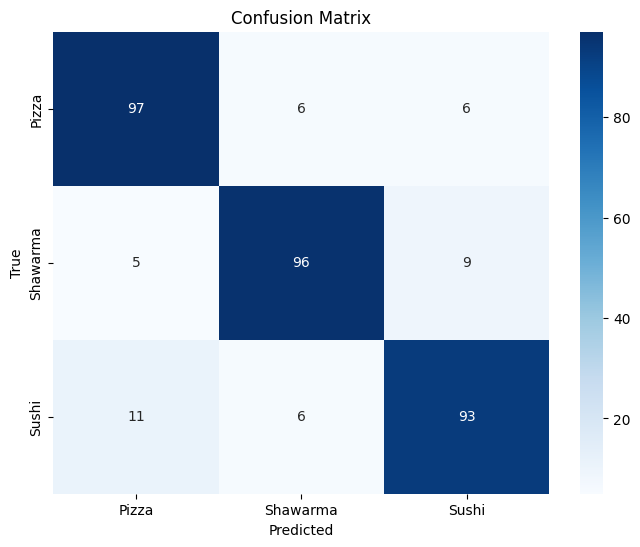
\includegraphics[width=0.45\textwidth]{model/neuralnetwork_confusion.png}
    \caption{Word Embedding Neural Network}
\end{table}

\subsection{Word Embedding - Linear Regression}
We also evaluated a linear regression model. The implementation leveraged sklearn's Linear Regression module, utilizing the same feature set as the neural network. The model achieved a validation accuracy of approximately 86\%, demonstrating competitive performance. This comparison with the neural network revealed that the simpler linear regression model performed slightly better, suggesting that the features representing the dataset may not exhibit significant complexity.

We tested multiple hyperparameter including setting `fit\_intercept' to False and `positive' to False. Setting `fit\_intercept' to False resulted in a lower accuracy of 0.85\%, while setting `positive' to False yielded the same accuracy as the default setting.

\begin{table}[h]
    \centering
    \begin{tabular}{lccc}
        \hline
        Category     & Precision                              & Recall & F1-score \\
        \hline
        Pizza        & 0.86                                   & 0.89   & 0.87     \\
        Shawarma     & 0.89                                   & 0.87   & 0.88     \\
        Sushi        & 0.86                                   & 0.85   & 0.85     \\
        \hline
        Accuracy     & \multicolumn{3}{c}{0.87 (329 samples)}                     \\
        Macro avg    & 0.87                                   & 0.87   & 0.87     \\
        Weighted avg & 0.87                                   & 0.87   & 0.87     \\
        \hline                                                                    \\
    \end{tabular}
    \begin{tabular}{ccc}
        \hline
        Loss   & Bias   & Variance \\
        \hline
        0.2515 & 0.2515 & 0.0088   \\
        \hline                     \\
    \end{tabular}
    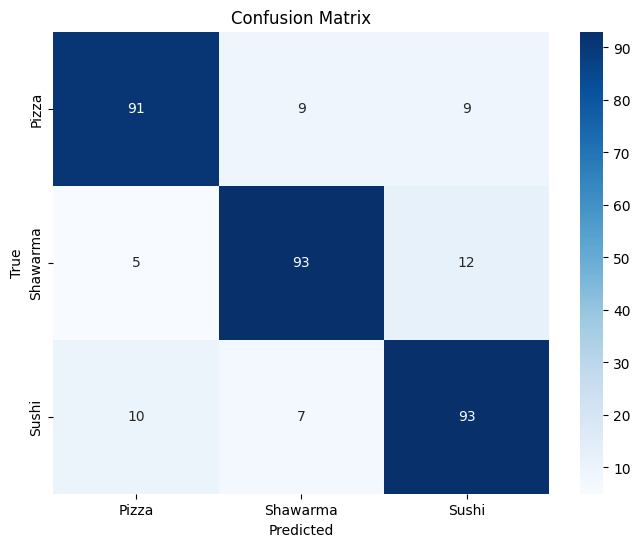
\includegraphics[width=0.45\textwidth]{model/linearregression_confusion.png}
    \caption{Word Embedding Linear Regression}
\end{table}

\subsection{Comparison of Word Embedding Models with Other Approaches}
The Word Embedding Neural Network yielded an accuracy of about 84\%, with a loss of 0.2269, a bias equal to its loss (0.2269), and a variance of 0.0731. The high bias suggests that it does not capture all complexity, while the variance stays relatively moderate. The Word Embedding Linear Regression achieved a slightly higher accuracy at 86\%, accompanied by a loss of 0.2515, bias of 0.2515, and a notably lower variance of 0.0088. Though its loss was higher, the overall bias-variance profile indicates more stable predictions compared to the neural network variant.

Compared to other models such as the MLPClassifier (90\% accuracy) and RandomForestClassifier (87\% accuracy), these word embedding approaches showed somewhat lower accuracies. The neural network had a higher variance component, while the regression model leaned toward higher bias. They both demonstrate that the selected text-based features might not require very deep representations, and simpler linear methods can yield competitive results. The neural network's complexity may not be justified given the representation of the dataset, as indicated by the performance of the linear regression model.

\section{Models}
% A description of the model(s) that you are evaluating/exploring. We are expecting a thorough
% exploration of at least 3+ family of models1, even if you don’t ultimately use those models. We are looking for:
% – How you are applying these models. You don’t need to reiterate what the models are and how they work. Instead, we’re looking for a description of the choices you are making to apply the model to this task: e.g., what features from the “Data” section are you using for each model? What adjustments (if any) did you need to make?

The setup of our training is similar for all models:
% Make a bullet point list
\begin{itemize}
\item We used the cleaned and encoded data as described in \ref{sec:exploration}.
\item We split the data into training, validation and test sets using a 60/20/20 split using \href{https://scikit-learn.org/stable/modules/generated/sklearn.model_selection.train_test_split.html}{train\_test\_split} from sklearn. We used a consistent random seed of 42 to ensure reproducibility.
\item We used stratified sampling to ensure that the distribution of classes is similar in both sets.
\item We used the same evaluation metrics for all models: accuracy, precision, recall, and F1-score.
\item We used \href{https://rasbt.github.io/mlxtend/user_guide/evaluate/bias_variance_decomp/}{bias\_variance\_decomp} from mlxtend to calculate the bias and variance of our models.
\item We used \href{https://scikit-learn.org/stable/modules/generated/sklearn.metrics.classification_report.html}{classification\_report} from sklearn to generate the classification report for our models.

\subsection{Neural Network}

We started with training a MLPClassifier on the cleaned and encoded data as described in \ref{sec:exploration} using the default parameters by
\href{https://scikit-learn.org/stable/modules/generated/sklearn.neural_network.MLPClassifier.html}{sklearn}.
The default configuration is as follows:
Hidden layer: 1 layer, 100 hidden units
Activation: ReLu
We achieved an 90\% validation accuracy with this base configuration without any tuning, and 87\% on the test set.
We have also tested bagged models and normalization. Specifically, we used the sklearn \href{https://scikit-learn.org/stable/modules/generated/sklearn.ensemble.BaggingClassifier.html}{BaggingClassifier}
with MLPClassifier as the estimator with 10 estimators. As we learned in class, we expected the bagged model to have lower variance because the prediction is the average of many MLPClassifiers.
This is confirmed when we performed variance bias decomposition as seen in \ref{tab:nn_bias_var}, where the bagged model has a lower variance than the non-bagged model.
We also tried normalizing the data using the \href{https://scikit-learn.org/stable/modules/generated/sklearn.preprocessing.StandardScaler.html}{StandardScaler} from sklearn.
We expected normalization to help the model converge faster and prevent overfitting, but it did not have a significant impact on the model accuracy.
We think this is because the data was already cleaned and encoded, and the features were already in a similar range.
For example, the numerical features like "How much would you expect to pay" already have similar ranges (5-20) as the categorical features like "How many ingredients would you expect to be in the food".

\begin{table}[ht]
    \centering
    \begin{tabular}{lccc}
        \hline
        Model                  & Expected Loss & Bias   & Variance \\
        \hline
        MLP                    & 0.1356        & 0.1155 & 0.0638   \\
        Bagging MLP            & 0.1362        & 0.1277 & 0.0543   \\
        Normalized MLP         & 0.1368        & 0.1185 & 0.0628   \\
        Normalized Bagging MLP & 0.1384        & 0.1337 & 0.0530   \\
        \hline
    \end{tabular}
    \caption{Loss, Bias, and Variance for Different Models}
    \label{tab:nn_bias_var}
\end{table}

\ref{tab:nn_classification_report} shows the classification report for the MLPClassifier.
The model performed well on the validation set, with an accuracy of 90\% and a balanced precision and recall across all classes.
The F1-score for all classes was around 0.90, indicating a good balance between precision and recall.

\begin{table}[ht]
    \centering
    \begin{tabular}{lcccc}
        \hline
        Category     & Precision & Recall & F1-score & Support \\
        \hline
        Pizza        & 0.92      & 0.90   & 0.91     & 88      \\
        Shawarma     & 0.87      & 0.91   & 0.89     & 88      \\
        Sushi        & 0.91      & 0.89   & 0.90     & 87      \\
        \hline
        Accuracy     &           &        & 0.90     & 263     \\
        Macro avg    & 0.90      & 0.90   & 0.90     & 263     \\
        Weighted avg & 0.90      & 0.90   & 0.90     & 263     \\
        \hline
    \end{tabular}
    \caption{Classification Report for Pizza, Shawarma, and Sushi}
    \label{tab:nn_classification_report}
\end{table}


\subsection{Decision Trees}
I tested a regular decision tree, an ensemble of decision trees, and a Random Forest model, using the built-in RandomForestClassifier from sklearn. I found the decision tree to perform the worst, and it was easier to manipulate the RandomForestClassifier’s parameters, so I decided to explore that further.

I decided to include all of the possible features (even initially 'id' accidentally), as the Random Forest was very robust regardless of the feature choice or hyperparameters. To allow the text-based features to generalize as well as possible, I used a library to cluster text by Levenshtein distance, and to limit overfitting, I only included the categories with enough representatives. This did not seem to have too large an impact on validation accuracy, but would allow it to correctly categorize otherwise unseen data with unique typos or spelling choices.
I tested many of the hyperparameter options, but found little change in accuracy aside from increasing the number of estimators to around 250, and limiting the minimum samples split to 10. Some randomness was introduced when generating text clusters, but I found it to still be very consistently accurate regardless of what data it trained on.

It consistently achieved an 87\% validation accuracy. The classification report initially showed it was particularly effective at identifying Pizza and Shawarma, but had some difficulty with Sushi, which I would expect if respondents have less familiarity with Sushi. However, after splitting the training data such that there is the same amount of each in the training and validation portions, this was no longer the case.
\begin{table}[ht]
    \centering
    \begin{tabular}{lccc}
        \hline
        Category     & Precision                              & Recall & F1-score \\
        \hline
        Pizza        & 0.85                                   & 0.93   & 0.89     \\
        Shawarma     & 0.88                                   & 0.84   & 0.86     \\
        Sushi        & 0.90                                   & 0.86   & 0.88     \\
        \hline
        Accuracy     & \multicolumn{3}{c}{0.88 (263 samples)}                     \\
        Macro avg    & 0.88                                   & 0.88   & 0.88     \\
        Weighted avg & 0.88                                   & 0.88   & 0.88     \\
        \hline
    \end{tabular}
    \caption{Classification Report}
    \label{tab:classification_report}
\end{table}

After comparing the loss, bias, variance decomposition to our other models, I found the expected higher bias, but lower variance that Random Forests are known to have:
\begin{table}[ht]
    \centering
    \begin{tabular}{ccc}
        \hline
        Loss   & Bias   & Variance \\
        \hline
        0.1380 & 0.1255 & 0.0410   \\
        \hline
    \end{tabular}
    \label{tab:loss_report}
\end{table}

\subsection{Word Embedding - Neural Network}
We implemented a feedforward neural network with three hidden layers consisting of 64, 64, and 64 neurons, respectively. The hidden layers utilized ReLU activation functions, while the output layer employed a softmax activation function. The model was trained using a learning rate of 0.001 and a batch size of 32, with categorical cross-entropy as the loss function. Training was conducted over 300 epochs, achieving a validation accuracy of approximately 84\%. For feature selection, we used word similarity embeddings for questions Q5, Q6, and Q7. For Q1, Q2, and Q4, we computed the average of all numerical values in the text, and for Q3 and Q8, we employed one-hot encoded categorical vectors.

We experimented with various configurations of the model, including adjustments to the number of hidden layers, neurons per layer, and activation functions. For activation functions, we tested leaky ReLU, sigmoid, and tanh. While leaky ReLU and tanh achieved validation accuracies of 82\% and 84\% respectively, the sigmoid function performed significantly worse, achieving only 65\%.

We also explored different hidden layer configurations. Increasing the number of neurons to 128, 64, and 64 per layer slightly reduced the accuracy to 82\% and increased training time. Reducing the neurons to 32, 16, and 16 per layer also resulted in a lower accuracy of 82\%. A configuration of 32 neurons in each of the three layers yielded a similar accuracy of 82\%.

Additionally, we tested varying the number of hidden layers while keeping each layer at 64 neurons. Reducing the number of layers to 1 or 2 led to validation accuracies of 82\% and 83\%, respectively. Increasing the number of layers to 4 or 5 did not improve performance, maintaining an accuracy of 84\%.

\begin{table}[h]
    \centering
    \begin{tabular}{lccc}
        \hline
        Category     & Precision                              & Recall & F1-score \\
        \hline
        Pizza        & 0.86                                   & 0.83   & 0.85     \\
        Shawarma     & 0.85                                   & 0.85   & 0.85     \\
        Sushi        & 0.82                                   & 0.85   & 0.83     \\
        \hline
        Accuracy     & \multicolumn{3}{c}{0.84 (329 samples)}                     \\
        Macro avg    & 0.84                                   & 0.84   & 0.84     \\
        Weighted avg & 0.84                                   & 0.84   & 0.84     \\
        \hline                                                                    \\
    \end{tabular}
    \begin{tabular}{ccc}
        \hline
        Loss   & Bias   & Variance \\
        \hline
        0.2269 & 0.2269 & 0.0731   \\
        \hline                     \\
    \end{tabular}
    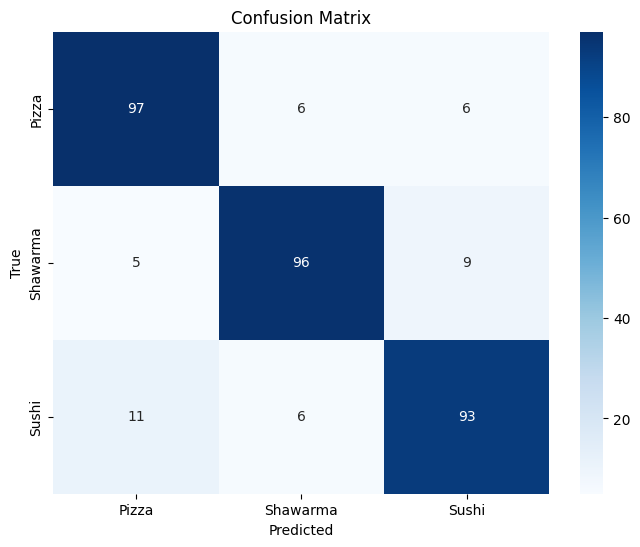
\includegraphics[width=0.45\textwidth]{model/neuralnetwork_confusion.png}
    \caption{Word Embedding Neural Network}
\end{table}

\subsection{Word Embedding - Linear Regression}
We also evaluated a linear regression model. The implementation leveraged sklearn's Linear Regression module, utilizing the same feature set as the neural network. The model achieved a validation accuracy of approximately 86\%, demonstrating competitive performance. This comparison with the neural network revealed that the simpler linear regression model performed slightly better, suggesting that the features representing the dataset may not exhibit significant complexity.

We tested multiple hyperparameter including setting `fit\_intercept' to False and `positive' to False. Setting `fit\_intercept' to False resulted in a lower accuracy of 0.85\%, while setting `positive' to False yielded the same accuracy as the default setting.

\begin{table}[h]
    \centering
    \begin{tabular}{lccc}
        \hline
        Category     & Precision                              & Recall & F1-score \\
        \hline
        Pizza        & 0.86                                   & 0.89   & 0.87     \\
        Shawarma     & 0.89                                   & 0.87   & 0.88     \\
        Sushi        & 0.86                                   & 0.85   & 0.85     \\
        \hline
        Accuracy     & \multicolumn{3}{c}{0.87 (329 samples)}                     \\
        Macro avg    & 0.87                                   & 0.87   & 0.87     \\
        Weighted avg & 0.87                                   & 0.87   & 0.87     \\
        \hline                                                                    \\
    \end{tabular}
    \begin{tabular}{ccc}
        \hline
        Loss   & Bias   & Variance \\
        \hline
        0.2515 & 0.2515 & 0.0088   \\
        \hline                     \\
    \end{tabular}
    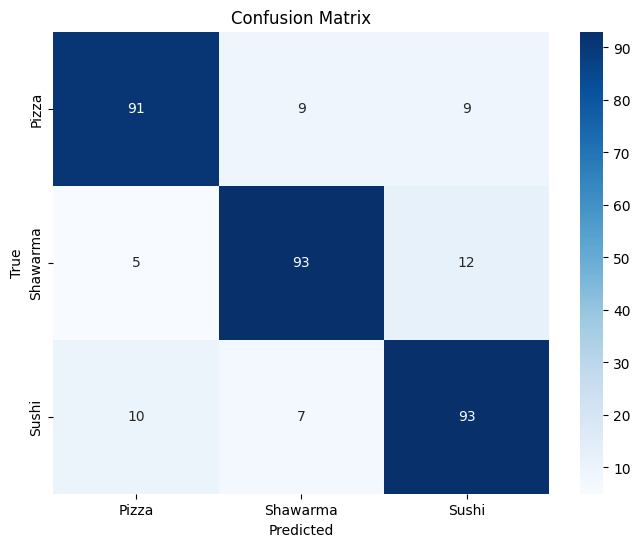
\includegraphics[width=0.45\textwidth]{model/linearregression_confusion.png}
    \caption{Word Embedding Linear Regression}
\end{table}

\subsection{Comparison of Word Embedding Models with Other Approaches}
The Word Embedding Neural Network yielded an accuracy of about 84\%, with a loss of 0.2269, a bias equal to its loss (0.2269), and a variance of 0.0731. The high bias suggests that it does not capture all complexity, while the variance stays relatively moderate. The Word Embedding Linear Regression achieved a slightly higher accuracy at 86\%, accompanied by a loss of 0.2515, bias of 0.2515, and a notably lower variance of 0.0088. Though its loss was higher, the overall bias-variance profile indicates more stable predictions compared to the neural network variant.

Compared to other models such as the MLPClassifier (90\% accuracy) and RandomForestClassifier (87\% accuracy), these word embedding approaches showed somewhat lower accuracies. The neural network had a higher variance component, while the regression model leaned toward higher bias. They both demonstrate that the selected text-based features might not require very deep representations, and simpler linear methods can yield competitive results. The neural network's complexity may not be justified given the representation of the dataset, as indicated by the performance of the linear regression model.

\section{Prediction}
% How well would you expect your model to perform on the test set? We are looking for:
% – A point estimate for your performance, not a range.
% – A reasoned explanation of your expected model performance, with empirical evidence supporting your explanation. You are not graded on the closeness of your estimate to the final test accuracy, but you are graded on your reasoning.
I would expect our model to perform with 80\% accuracy on the test set. Our separated test accuracy resulted in 86\%, and the test set the model will be predicting for is from a slightly different population, so it is reasonable to expect less accuracy.
The given dataset and the test set however should be similar, and testing how it performs on less correlated data does give an idea as to how it may perform here. We have also tested the model on synthetic datasets generated by AIs and programatically, and found promising results to support the idea that the model has generalized well.

\begin{figure}[h]
  \centerline{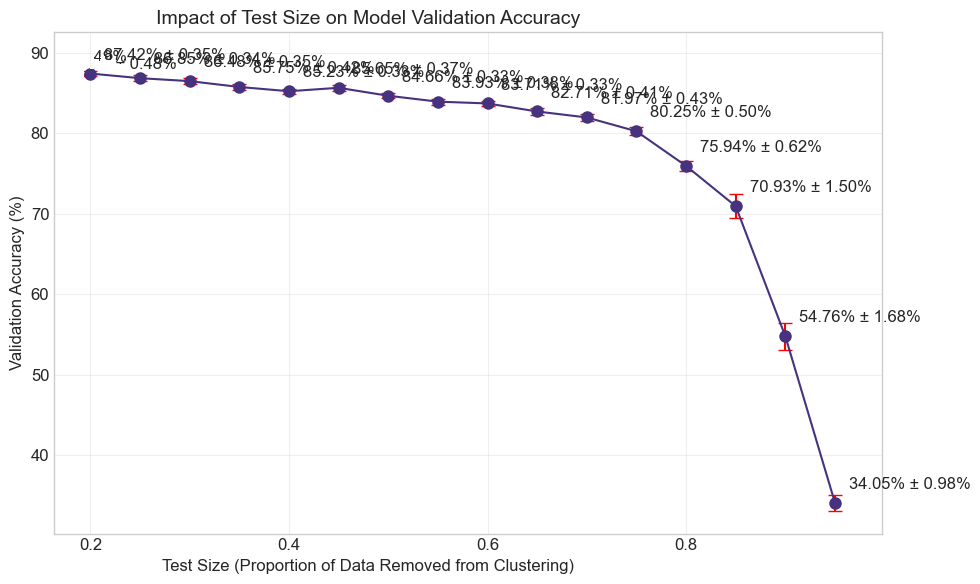
\includegraphics[width=\columnwidth]{TestSize.png}}
  \caption{Impact of smaller dataset on Validation Accuracy}
  \label{f:testsize_diagram}
\end{figure}


\section{Workload Distribution}
% A description of what each person in the group contributed to the project. A 1-2 sentence description of each person’s role is sufficient. Each student’s description must be written by that
% student in order for them to receive credit for the project.

Ryan Shiels worked on the data cleaning and input functions, and explored Decision Trees/Random Forest models.\\
Siqi Liu: data visualization and implementing the MLP Classifier\\
Rafay Usman: data cleaning and implementing/tuning the MLP Classifier\\
Albert Li\\

\end{document}
